% Kenapa ESP32 + chip FPGA, bukan komputer mini (Raspberry Pi/SBC) seperti sistem TA saat ini.
\documentclass[border=4pt]{standalone}
% Gaya bersama gambar deck Demo Day (dipakai semua gambar/*.tex standalone).
\usepackage{amssymb}
\usepackage{fontspec}
\setmainfont{DejaVu Sans Condensed}
\setsansfont{DejaVu Sans Condensed}
\newfontfamily\judulfont{DejaVu Sans}[BoldFont={DejaVu Sans Bold}, Ligatures=TeX]
\usepackage{tikz,pgfplots}
\pgfplotsset{compat=1.18, every axis/.append style={/pgf/number format/assume math mode=true, /pgf/number format/use comma, /pgf/number format/1000 sep={.}}}
\usetikzlibrary{positioning,arrows.meta,calc,shapes.geometric,fit,backgrounds}
\definecolor{gelap}{HTML}{15242B}
\definecolor{teal}{HTML}{285052}
\definecolor{amber}{HTML}{E8A317}
\definecolor{muda}{HTML}{DCE8E8}
\definecolor{abu}{HTML}{8A9499}
\definecolor{teks}{HTML}{1E2B30}
\definecolor{hijau}{HTML}{2F7D5B}
\definecolor{merah}{HTML}{A33A2A}
\color{teks}
\tikzset{
  ubin/.style={fill=muda, rounded corners=5pt, align=center, inner sep=6pt},
  inti/.style={ubin, fill=gelap, text=white},
  panah/.style={-{Stealth[length=3mm]}, line width=1.3pt, draw=amber},
  panahabu/.style={-{Stealth[length=2.5mm]}, line width=1pt, draw=abu},
  judulubin/.style={font=\judulfont\bfseries},
}
% Dibuat otomatis oleh buat_aset.py dari ml/results/energi_harian.json; jangan diedit manual.
\newcommand{\energiTurbin}{270}
\newcommand{\energiQa}{187}
\newcommand{\energiQb}{377}
\newcommand{\hariEnergi}{140}
\newcommand{\raspiWh}{71}
\newcommand{\chipWh}{4,1}
\newcommand{\raspiPersen}{26}
\newcommand{\chipPersen}{1,5}
\newcommand{\raspiPersenA}{19}
\newcommand{\raspiPersenB}{38}
\newcommand{\raspiPersenNum}{26.3}
\newcommand{\chipPersenNum}{1.5}
\newcommand{\hematKwh}{24}
\newcommand{\kaliHemat}{17}
\newcommand{\jRaspi}{182}
\newcommand{\jChip}{10,4}
\newcommand{\periodeEnergi}{2026-03-31--2026-10-20}

\AtBeginDocument{\hyphenpenalty=10000 \exhyphenpenalty=10000}

\begin{document}
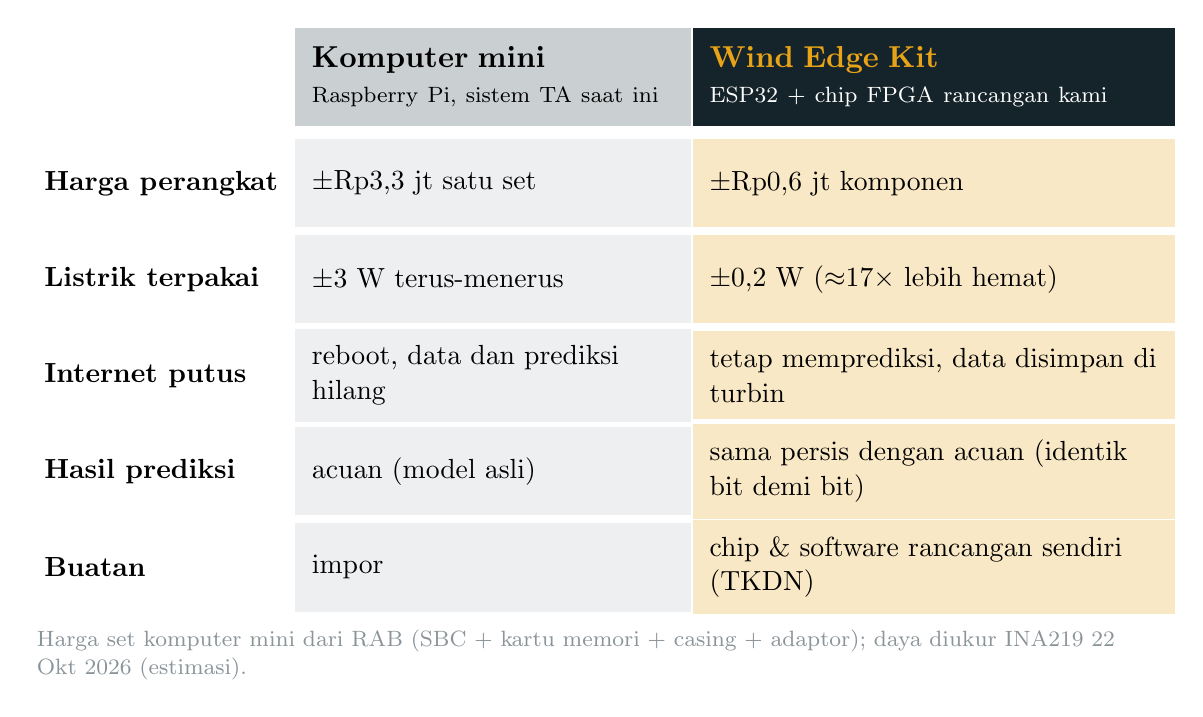
\begin{tikzpicture}[font=\fontsize{10}{12.5}\selectfont,
  sel/.style={minimum height=1.12cm, text width=#1, align=left, inner sep=6pt, anchor=west}]
  \def\baris#1#2#3#4{%
    \node[sel=3.1cm, font=\bfseries\fontsize{10}{12.5}\selectfont] at (0,#1) {#2};
    \node[sel=4.6cm, fill=abu!15] at (3.4,#1) {#3};
    \node[sel=5.7cm, fill=amber!25] at (8.45,#1) {#4};}
  \node[sel=4.6cm, fill=abu!45, minimum height=1.25cm] at (3.4,1.35) {{\judulfont\bfseries\fontsize{10.5}{13}\selectfont Komputer mini}\\{\fontsize{8.5}{10}\selectfont Raspberry Pi, sistem TA saat ini}};
  \node[sel=5.7cm, fill=gelap, text=white, minimum height=1.25cm] at (8.45,1.35) {{\judulfont\bfseries\fontsize{10.5}{13}\selectfont\color{amber}Wind Edge Kit}\\{\fontsize{8.5}{10}\selectfont ESP32 + chip FPGA rancangan kami}};
  \baris{0}{Harga perangkat}{$\pm$Rp3,3 jt satu set}{$\pm$Rp0,6 jt komponen}
  \baris{-1.22}{Listrik terpakai}{$\pm$3 W terus-menerus}{$\pm$0,2 W ($\approx$17$\times$ lebih hemat)}
  \baris{-2.44}{Internet putus}{reboot, data dan prediksi hilang}{tetap memprediksi, data disimpan di turbin}
  \baris{-3.66}{Hasil prediksi}{acuan (model asli)}{sama persis dengan acuan (identik bit demi bit)}
  \baris{-4.88}{Buatan}{impor}{chip \& software rancangan sendiri (TKDN)}
  \node[anchor=north west, text=abu, font=\fontsize{8}{10}\selectfont, text width=14.2cm] at (0,-5.55)
    {Harga set komputer mini dari RAB (SBC + kartu memori + casing + adaptor); daya diukur INA219 22 Okt 2026 (estimasi).};
\end{tikzpicture}
\end{document}
